\documentclass[11pt,compress,t,notes=noshow]{beamer}
\usepackage[]{graphicx}\usepackage[]{color}
% maxwidth is the original width if it is less than linewidth
% otherwise use linewidth (to make sure the graphics do not exceed the margin)
\makeatletter
\def\maxwidth{ %
  \ifdim\Gin@nat@width>\linewidth
    \linewidth
  \else
    \Gin@nat@width
  \fi
}
\makeatother

\definecolor{fgcolor}{rgb}{0.345, 0.345, 0.345}
\newcommand{\hlnum}[1]{\textcolor[rgb]{0.686,0.059,0.569}{#1}}%
\newcommand{\hlstr}[1]{\textcolor[rgb]{0.192,0.494,0.8}{#1}}%
\newcommand{\hlcom}[1]{\textcolor[rgb]{0.678,0.584,0.686}{\textit{#1}}}%
\newcommand{\hlopt}[1]{\textcolor[rgb]{0,0,0}{#1}}%
\newcommand{\hlstd}[1]{\textcolor[rgb]{0.345,0.345,0.345}{#1}}%
\newcommand{\hlkwa}[1]{\textcolor[rgb]{0.161,0.373,0.58}{\textbf{#1}}}%
\newcommand{\hlkwb}[1]{\textcolor[rgb]{0.69,0.353,0.396}{#1}}%
\newcommand{\hlkwc}[1]{\textcolor[rgb]{0.333,0.667,0.333}{#1}}%
\newcommand{\hlkwd}[1]{\textcolor[rgb]{0.737,0.353,0.396}{\textbf{#1}}}%
\let\hlipl\hlkwb

\usepackage{framed}
\makeatletter
\newenvironment{kframe}{%
 \def\at@end@of@kframe{}%
 \ifinner\ifhmode%
  \def\at@end@of@kframe{\end{minipage}}%
  \begin{minipage}{\columnwidth}%
 \fi\fi%
 \def\FrameCommand##1{\hskip\@totalleftmargin \hskip-\fboxsep
 \colorbox{shadecolor}{##1}\hskip-\fboxsep
     % There is no \\@totalrightmargin, so:
     \hskip-\linewidth \hskip-\@totalleftmargin \hskip\columnwidth}%
 \MakeFramed {\advance\hsize-\width
   \@totalleftmargin\z@ \linewidth\hsize
   \@setminipage}}%
 {\par\unskip\endMakeFramed%
 \at@end@of@kframe}
\makeatother

\definecolor{shadecolor}{rgb}{.97, .97, .97}
\definecolor{messagecolor}{rgb}{0, 0, 0}
\definecolor{warningcolor}{rgb}{1, 0, 1}
\definecolor{errorcolor}{rgb}{1, 0, 0}
\newenvironment{knitrout}{}{} % an empty environment to be redefined in TeX

\usepackage{alltt}
\newcommand{\SweaveOpts}[1]{}  % do not interfere with LaTeX
\newcommand{\SweaveInput}[1]{} % because they are not real TeX commands
\newcommand{\Sexpr}[1]{}       % will only be parsed by R



\usepackage[english]{babel}
\usepackage{dsfont}
\newcommand\bmmax{2}
\usepackage{bm}
\usepackage{bbm}
\usepackage{verbatim}
\usepackage{amsmath}
\usepackage{amsfonts}
\usepackage{csquotes}
\usepackage{multirow}
\usepackage{longtable}
\usepackage{enumerate}
\usepackage[absolute,overlay]{textpos}
\usepackage{psfrag}
\usepackage{algorithm}
\usepackage{algorithmicx}
\usepackage{algpseudocode}
\usepackage{eqnarray}
\usepackage{multimedia}
\usepackage{media9}
\usepackage{arydshln}
\usepackage{tabularx}
\usepackage{placeins}
\usepackage{tikz}
\usepackage{setspace}
\usepackage{wrapfig}
\usepackage{tcolorbox}
\usepackage[export]{adjustbox}
\usepackage{siunitx}
\usetikzlibrary{shapes,arrows,automata,positioning,calc}
\def\signed #1{{\leavevmode\unskip\nobreak\hfil\penalty50\hskip1em
  \hbox{}\nobreak\hfill #1%
  \parfillskip=0pt \finalhyphendemerits=0 \endgraf}}

\newsavebox\mybox
\newenvironment{aquote}[1]
  {\savebox\mybox{#1}\begin{quote}\openautoquote\hspace*{-.7ex}}
  {\unskip\closeautoquote\vspace*{1mm}\signed{\usebox\mybox}\end{quote}}
  
\tikzset{
  %Define standard arrow tip
  >=stealth',
  %Define style for boxes
  punkt/.style={
    rectangle,
    rounded corners,
    draw=black, very thick,
    text width=6.5em,
    minimum height=2em,
    text centered},
  % Define arrow style
  pil/.style={
    ->,
    thick,
    shorten <=2pt,
    shorten >=2pt,}
}
\usepackage{subfig}

%new environments

\newenvironment{vbframe}  %frame with breaks and verbatim
{
 \begin{frame}[containsverbatim,allowframebreaks]
}
{
\end{frame}
}

\newenvironment{vframe}  %frame with verbatim without breaks (to avoid numbering one slided frames)
{
 \begin{frame}[containsverbatim]
}
{
\end{frame}
}

\newenvironment{blocki}[1]   % itemize block
{
 \begin{block}{#1}\begin{itemize}
}
{
\end{itemize}\end{block}
}

\newenvironment{fragileframe}[2]{  %fragile frame with framebreaks
\begin{frame}[allowframebreaks, fragile, environment = fragileframe]
\frametitle{#1}
#2}
{\end{frame}}


\newcommand{\myframe}[2]{  %short for frame with framebreaks
\begin{frame}[allowframebreaks]
\frametitle{#1}
#2
\end{frame}}

\newcommand{\remark}[1]{
  \textbf{Remark:} #1
}

%%%%%%%%%%%%%%%%%%%%%%%%%%%%%%%%%%%%%%%%%%%%%%%%%%%%%%%%%%%%%%%%%%%%%%%%%%%%%%%

% basic latex stuff
\newcommand{\pkg}[1]{{\fontseries{b}\selectfont #1}} %fontstyle for R packages
\newcommand{\lz}{\vspace{0.5cm}} %vertical space
\newcommand{\dlz}{\vspace{1cm}} %double vertical space
\newcommand{\oneliner}[1] % Oneliner for important statements
{\begin{block}{}\begin{center}\begin{Large}#1\end{Large}\end{center}\end{block}}


%\usetheme{lmu-lecture}
\usepackage{../style/lmu-lecture}

\let\code=\texttt
\let\proglang=\textsf

\setkeys{Gin}{width=0.9\textwidth}



\title{Introduction to Machine Learning}
\author{Bernd Bischl}
\institute{Department of Statistics -- LMU Munich}
\date{Winter term 2021}

\setbeamertemplate{frametitle}{\expandafter\uppercase\expandafter\insertframetitle}



\begin{document}




\input{../latex-math/basic-math}
\input{../latex-math/basic-ml}
\input{../latex-math/ml-nn}

\lecturechapter{1}{Deep Learning- History of Neural Networks}
\lecture{Deep Learning- History of Neural Networks}
%%%%%%%%%%%%%%%%%%%%%%%%%%%%%%%%%%%%%%%%%%%%%%%%%%%%%%%%%%%%%%%%%%

\begin{vbframe}{A brief history of neural networks}
\begin{itemize}
\item \pkg{1943:} The first artificial neuron, the "Threshold Logic Unit (TLU)", was proposed by Warren McCulloch \& Walter Pitts.
\begin{figure}
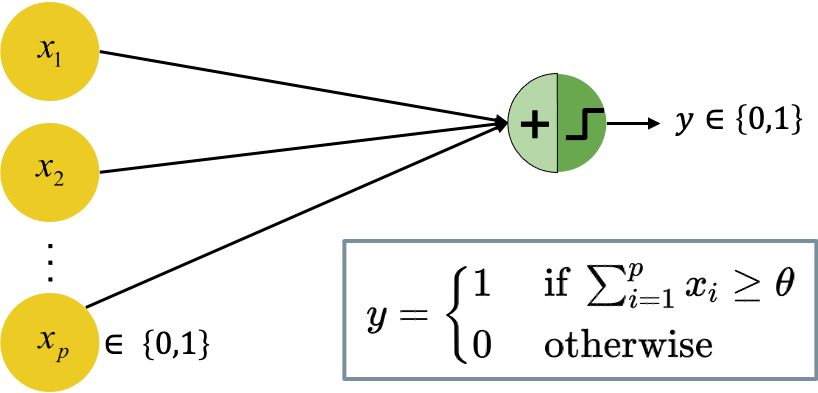
\includegraphics[width=7cm]{plots/mp_neuron.png}
\end{figure}
\begin{itemize}
\item In this model the neuron fires a $+1$ if the input exceeds a certain threshold $\theta$.
\vspace{2mm}
\item However, this model did not have adjustable weights, so learning could only be achieved by changing the threshold $\theta$.
\end{itemize}
\end{itemize}
\framebreak
%%%%%%%%%%%%%%%%%%%%%%%%%%%%%%%%%%%%%%%%%%%%%%%%%%%%%%%%%%%%%%%%%%  

\begin{itemize}
\item \pkg{1957:} The perceptron was invented by Frank Rosenblatt. 
\begin{figure}
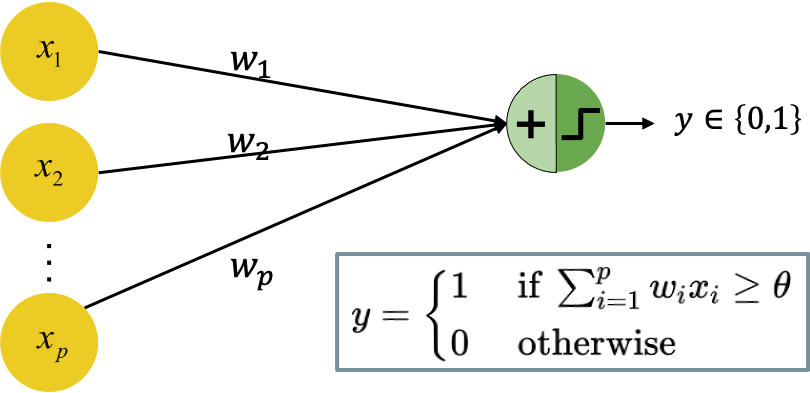
\includegraphics[width=7cm]{plots/perceptron_new.png}
\end{figure}
\begin{itemize}
\item In perceptron, the weights are adjustable and can be learned by learning algorithms. 
\vspace{2mm}
\item The inputs are not restricted to be binary.
\vspace{2mm}
\item Similar to the MP-neuron, the threshold is adjustable, and decision boundaries are linear.
\end{itemize}
\end{itemize}
\framebreak
%%%%%%%%%%%%%%%%%%%%%%%%%%%%%%%%%%%%%%%%%%%%%%%%%%%%%%%%%%%%%%%%%%

\begin{itemize}
\item \pkg{1960:} ADALINE by Bernard Widrow \& Ted Hoff; weights are now adjustable according to the weighted sum of the inputs.
\vspace{.1cm}
\begin{figure}
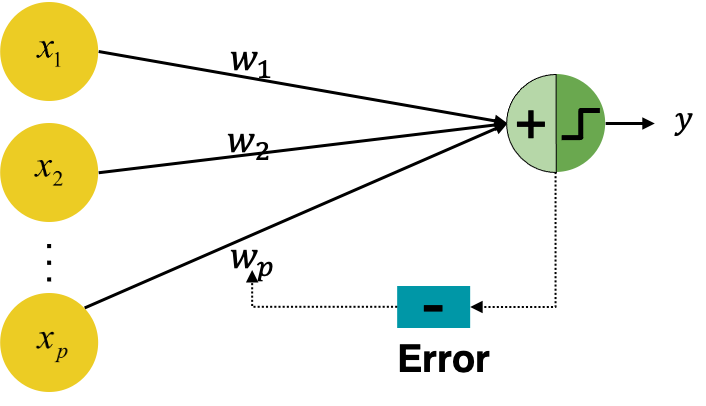
\includegraphics[width=7cm]{plots/adaline.png}
\end{figure}
\vspace{1cm}
\item \pkg{1965:} Group method of data handling (also known as polynomial neural networks) by Alexey Ivakhnenko. The first learning algorithm for supervised deep feedforward multilayer perceptrons.
\framebreak
%%%%%%%%%%%%%%%%%%%%%%%%%%%%%%%%%%%%%%%%%%%%%%%%%%%%%%%%%%%%%%%%%%

\item \pkg{1969:} The first \enquote{AI Winter} kicked in.
\begin{itemize}
\item Marvin Minsky \& Seymour Papert proved that a perceptron cannot solve the XOR-Problem (linear separability).
\item Less funding $\Rightarrow$ Standstill in AI/DL research
\end{itemize}
\end{itemize}
\begin{figure}
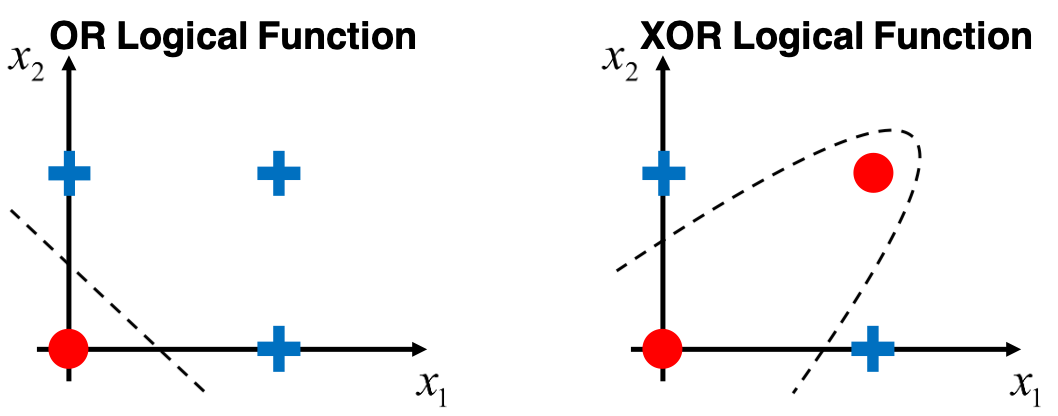
\includegraphics[width=7cm]{plots/orvsxor.png}
\end{figure}
\begin{itemize}
\item \pkg{1985:} Multi-layered perceptron with backpropagation by David Rumelhart, Geoffrey Hinton and Ronald Williams.
\begin{itemize}
\item Efficiently compute derivatives of composite functions.
\item Backpropagation was developed already in 1970 by Linnainmaa.
\end{itemize}
\framebreak
%%%%%%%%%%%%%%%%%%%%%%%%%%%%%%%%%%%%%%%%%%%%%%%%%%%%%%%%%%%%%%%%%%

\item \pkg{1985:} The second \enquote{AI Winter} kicked in.
\begin{itemize}
\item Overly optimistic/exaggerated expectations concerning potential of AI/DL.
\item Angering investors, the phrase \enquote{AI} even reached a pseudoscience status.
\item Kernel machines and graphical models both achieved good results on many important tasks.
\item Some of the fundamental mathematical difficulties in modeling long sequences were identified.
\end{itemize}
\begin{figure}
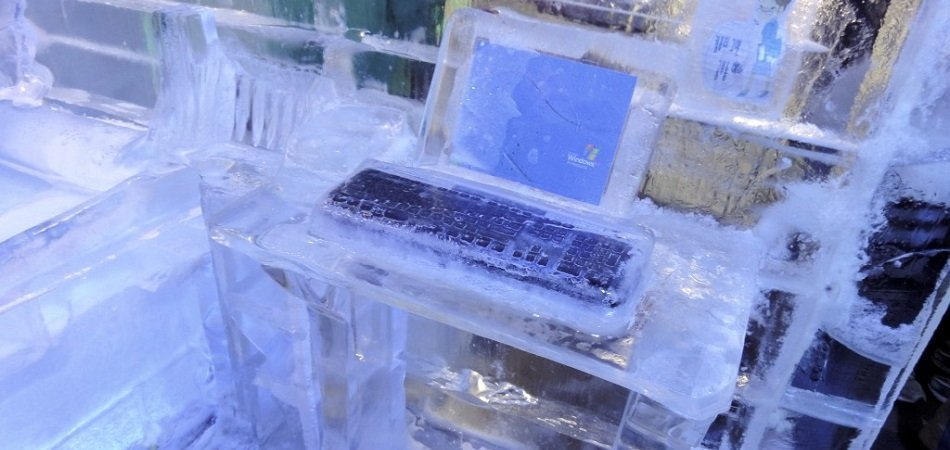
\includegraphics[width=7cm]{plots/ai_winter.jpg}
\end{figure}
\framebreak
%%%%%%%%%%%%%%%%%%%%%%%%%%%%%%%%%%%%%%%%%%%%%%%%%%%%%%%%%%%%%%%%%%

\item \pkg{2006:} Age of deep neural networks began.
\begin{itemize}
\item Geoffrey Hinton showed that a deep belief network could be efficiently trained using \textit{greedy layer-wise pretraining}.
\item This wave of research popularized the use of the term deep learning to emphasize that researchers were now able to train deeper neural networks than had been possible before.
\item At this time, deep neural networks outperformed competing AI systems based on other ML technologies as well as hand-designed functionality.
\end{itemize}
\begin{figure}
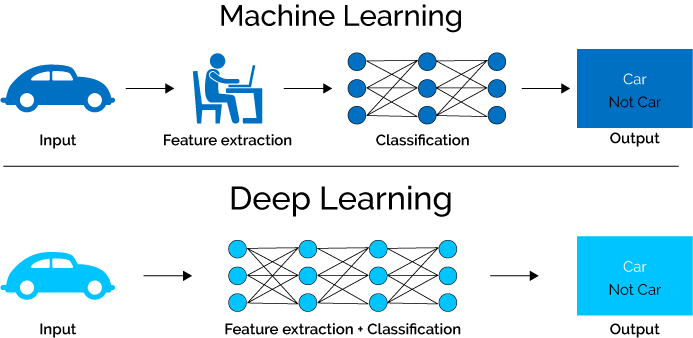
\includegraphics[width=6.5cm]{plots/dl_feature2.png}
\end{figure}
\framebreak
%%%%%%%%%%%%%%%%%%%%%%%%%%%%%%%%%%%%%%%%%%%%%%%%%%%%%%%%%%%%%%%%%%

\textbf{Why now and not earlier?}
\begin{itemize}
\item Significantly bigger datasets.
\item Better algorithms and the vanishing gradient problem (optimization chapter).
\item Better regularization (regularization chapter).
\item Unsupervised representation learning (autoencoder chapter).
\item More layers inevitably lead to a significant increase of parameters.
\item Back then, processing power was simply not capable to handle such huge amounts of parameters.
$\Rightarrow$ Nowadays, deep neural networks are trained on GPUs (graphic processing units), not on CPUs (central processing units).
\item Investment by industries and universities.
\item Deep learning tools make learning and applying deep learning easier.
\end{itemize}
\end{itemize}
\framebreak
%%%%%%%%%%%%%%%%%%%%%%%%%%%%%%%%%%%%%%%%%%%%%%%%%%%%%%%%%%%%%%%%%%

\begin{figure}
\centering
\scalebox{1.1}{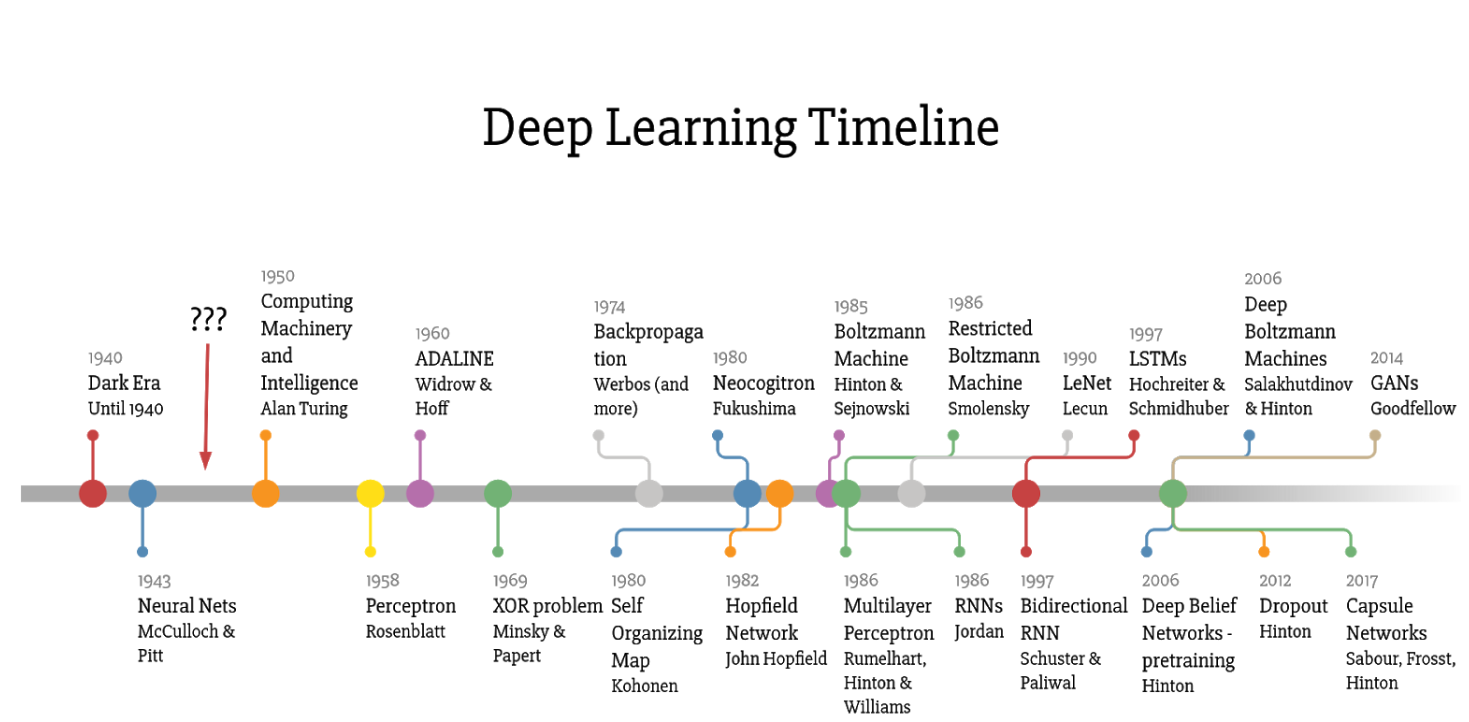
\includegraphics{plots/dl_timeline.png}}
\caption{Credit: Favio Vazquez}
\framebreak
%%%%%%%%%%%%%%%%%%%%%%%%%%%%%%%%%%%%%%%%%%%%%%%%%%%%%%%%%%%%%%%%%%

\scalebox{1.1}{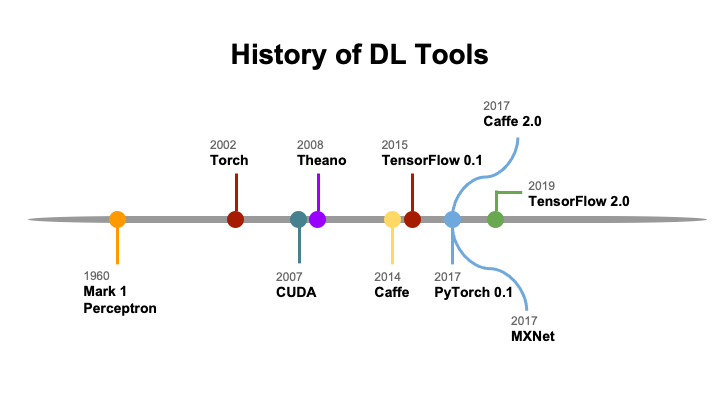
\includegraphics{plots/DL_tools.png}}
\end{figure}
\framebreak
%%%%%%%%%%%%%%%%%%%%%%%%%%%%%%%%%%%%%%%%%%%%%%%%%%%%%%%%%%%%%%%%%%

\begin{figure}
\centering
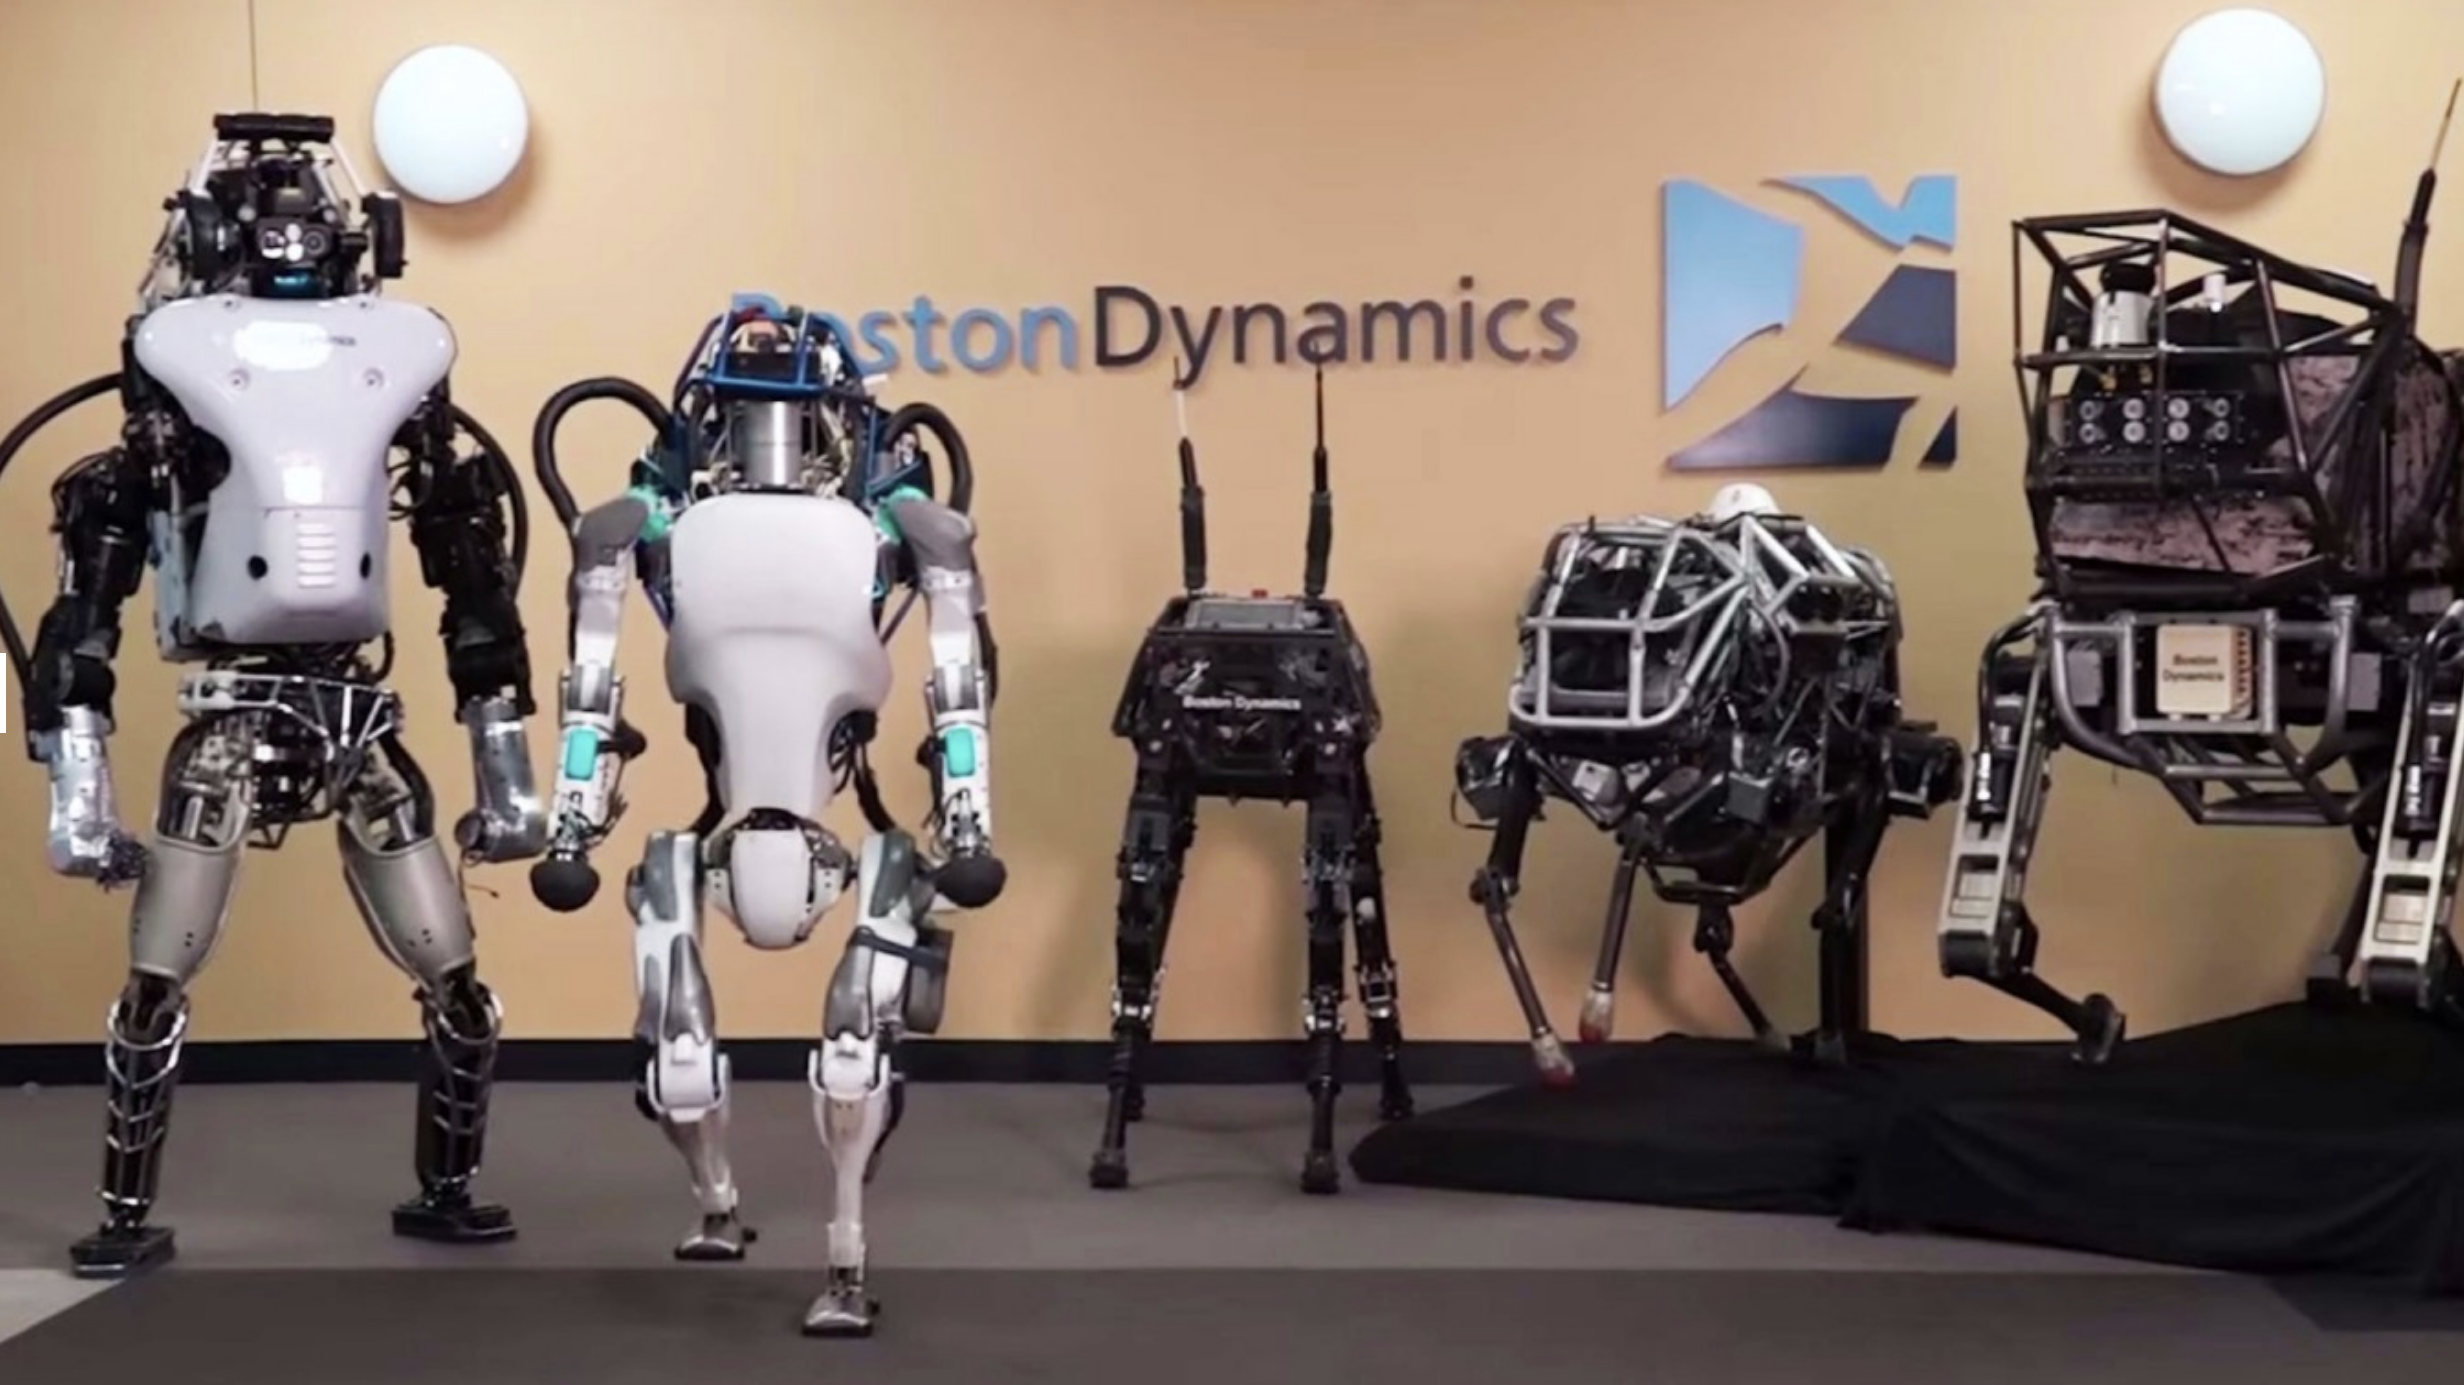
\includegraphics[width=8cm]{plots/bostondynamic.png}
\caption{Boston Dynamics (\href{https://www.youtube.com/watch?v=fUyU3lKzoio&ab_channel=BostonDynamics}{click here})}
\end{figure}
\footnotesize
\begin{itemize}
\item Boston Dynamics is a world leader in mobile robots founded in 1992 as a spin-off from the Massachusetts Institute of Technology.
\vspace{.1cm}
\item The company is best known for the development of a series of dynamic highly-mobile robots, including BigDog, Spot, Atlas, and Handle.
\end{itemize}
\framebreak
%%%%%%%%%%%%%%%%%%%%%%%%%%%%%%%%%%%%%%%%%%%%%%%%%%%%%%%%%%%%%%%%%%

\begin{figure}
\centering
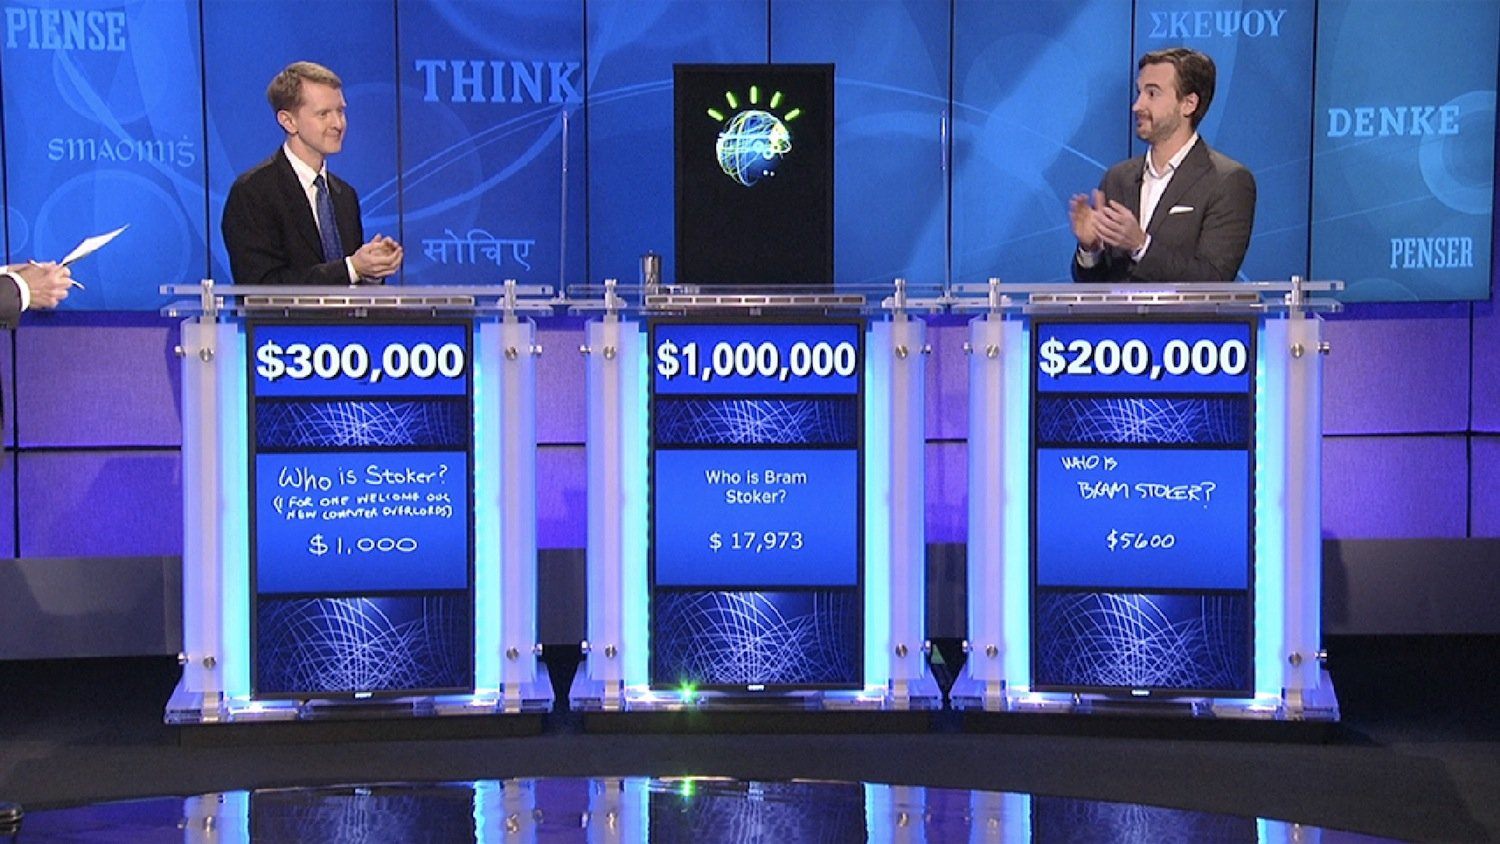
\includegraphics[width=8cm]{plots/ibmsupercomputer.jpg}
\caption{IBM Supercomputer}
\end{figure}
\footnotesize
\begin{itemize}
\item Watson is a question-answering system capable of answering questions posed in natural language, developed in IBM's DeepQA project.
\vspace{.1cm}
\item In 2011, Watson competed on \textit{Jeopardy!} against champions Brad Rutter and Ken Jennings, winning the first place prize of $\$ 1$ million.
\end{itemize}
\framebreak
%%%%%%%%%%%%%%%%%%%%%%%%%%%%%%%%%%%%%%%%%%%%%%%%%%%%%%%%%%%%%%%%%%

\begin{figure}
\centering
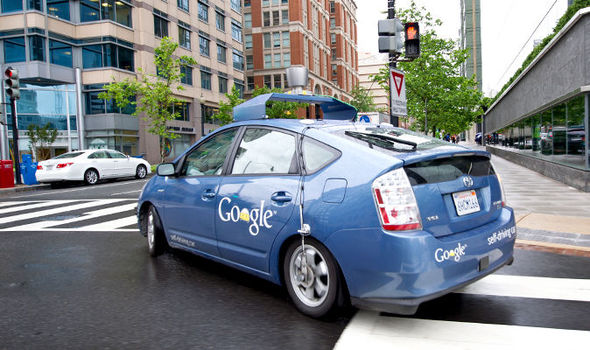
\includegraphics[width=8cm]{plots/selfdriving.jpg}
\caption{Google self driving car (Waymo)}
\end{figure}
\footnotesize
\begin{itemize}
\item Google's development of self-driving technology began on January 17, 2009, at the company's secretive X lab.
\vspace{.1cm}
\item By January 2020, $20$ million miles of self-driving on public roads had been completed by Waymo.
\end{itemize}
\end{vbframe}
%%%%%%%%%%%%%%%%%%%%%%%%%%%%%%%%%%%%%%%%%%%%%%%%%%%%%%%%%%%%%%%%%%

\endlecture
\end{document}
